\section{Implementace}
Nyní když máme všechen návrh i analýzu hotovou, můžeme se pustit do implementace. V této kapitole se zaměříme na konkrétní implementaci API pro naši hru.

\subsection{Nastavení projektu}

Pokud máte IntelliJ IDEA ultimate, máte možnost vytvořit nový projekt Spring Boot. Pokud ne, můžete použít Spring Initializer, což je webová aplikace, která vám umožní vytvořit nový projekt Spring Boot.
Pokud nemáte tak můžete navštívit Spring Initializer \url{https://start.spring.io/} a přidejte následující závislosti do projektu:

\begin{itemize}
    \item Spring Web
    \item Spring Data JPA
    \item H2 Database
\end{itemize}

Můžete přidat do projektu i další velice užitečné závislosti.
\begin{itemize}
    \item Lombok - snižuje množství kódu, který musíte napsat
    \item Spring HATEOAS - umožňuje jednodušeji vytvářet url odkazy
\end{itemize}

Místo H2 databáze můžete použít jakoukoli jinou databázi, která je podporována Spring Boot. Ovšem H2 je velice jednoduchá databáze, která je pouze v paměti (H2 in-memory database), což je ideální pro demonstrování. Ovšem to nemění nic na implementaci API, která je stejná pro jakoukoli jinou databázi.

Změňte název projektu a poté vyberte "Generate". Stáhne se .zip soubor, který se musí rozbalit. Uvnitř najdete jednoduchý projekt založený na Maven, včetně souboru pom.xml (Poznámka: Můžete použít i Gradle, ale příklady v tomto příkladu budou založeny na Maven).

Spring Boot funguje s jakýmkoli IDE, můžete použít Eclipse, IntelliJ IDEA, Netbeans, atd.

Pro automaticky generovanou dokumentaci můžete přidat závislost Springdoc Swagger 2 (viz. \ref{code:swagger-dependency}). Tato závislost se přidává do souboru \texttt{pom.xml} v kořeni projektu.
Poté můžete spustit projekt a zobrazí se vám dokumentace na adrese \url{http://localhost:8080/swagger-ui/index.html}.

\begin{listing}[H]
    \begin{minted}{xml}
        <!-- https://mvnrepository.com/artifact/org.springdoc/springdoc-openapi-ui -->
        <dependency>
            <groupId>org.springdoc</groupId>
            <artifactId>springdoc-openapi-starter-webmvc-ui</artifactId>
            <version>2.2.0</version>
        </dependency>
    \end{minted}
    \caption{Přidání závislosti Springdoc Swagger 2}
    \label{code:swagger-dependency}
\end{listing}

\begin{figure}[H]
    \centering
    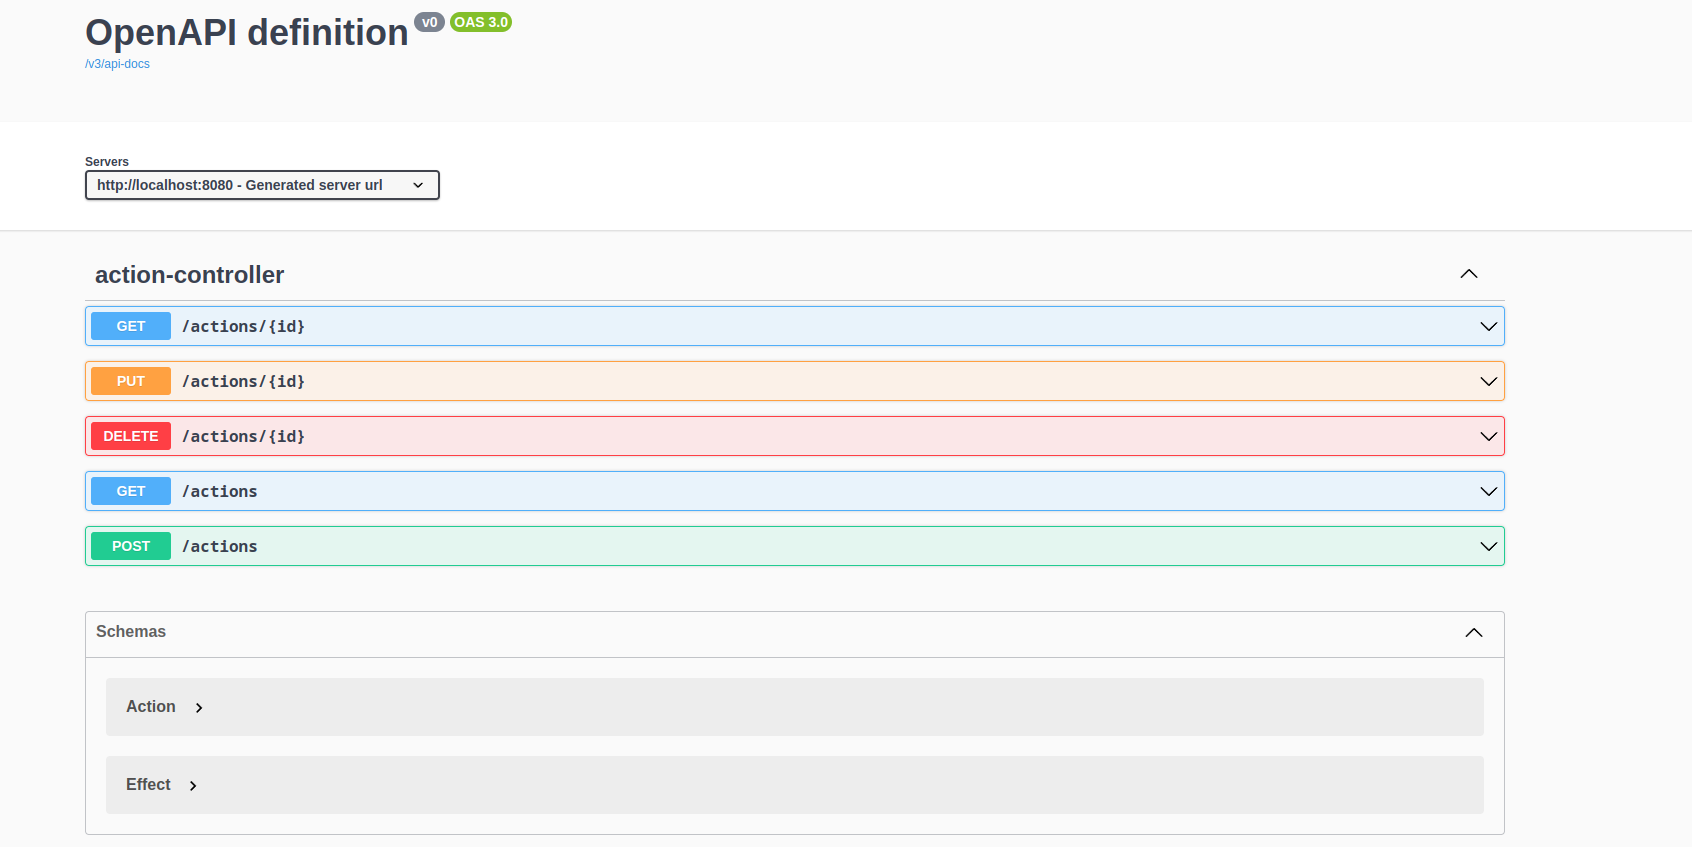
\includegraphics[width=0.9\textwidth]{../images/implementation/swagger.png}
    \caption{rozhraní Swagger}
    \label{fig:swagger-ui}
\end{figure}
\begin{figure}[H]
    \centering
    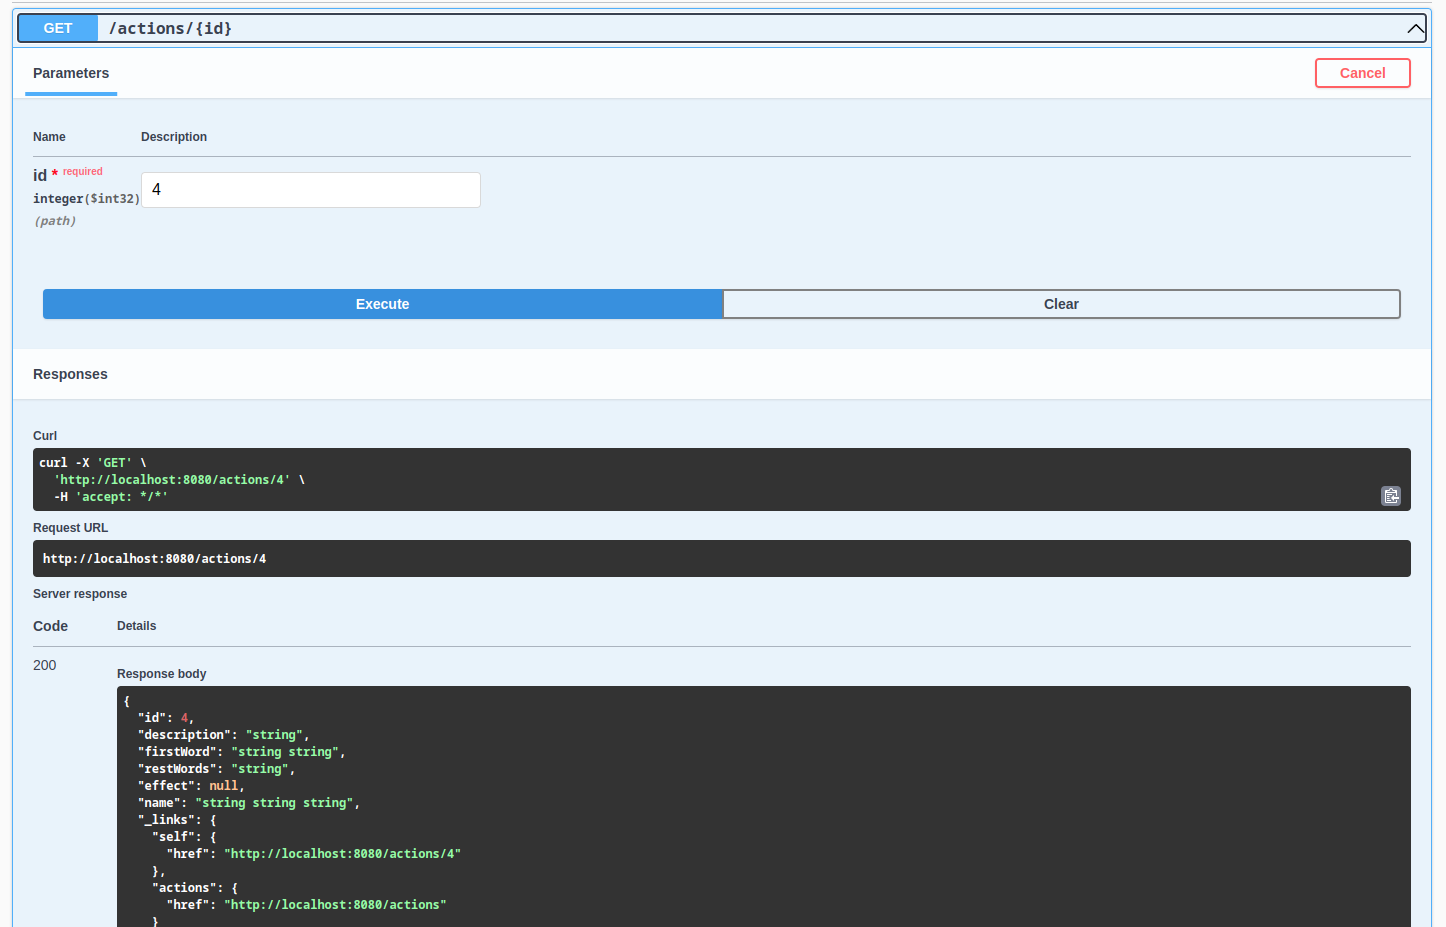
\includegraphics[width=0.9\textwidth]{../images/implementation/swaggger endpoint.png}
    \caption{Detail konkrétního endpointu}
    \label{fig:swagger-ui}
\end{figure}


\subsection{Vytvoření kostry}
Následně se podíváme na věci, které je třeba udělat pro úplné minimum funkčnosti API. Vytvoříme entitu, repository a načteme nějaké výchozí data a vytvoříme jednoduchý controller.

První věc, kterou musíme udělat, je vytvořit entitu. Entita je třída, která reprezentuje tabulku v databázi. V našem případě budeme mít entitu pro Akci a entitu pro Efekt akce.

\begin{listing}[H]
    \begin{minted}{java}
@Data
@Entity
@NoArgsConstructor
@AllArgsConstructor
@Builder(toBuilder = true)
public class Action {
    @Id @GeneratedValue(strategy = GenerationType.AUTO)
    private Integer id;

    private String name;

    @NonNull @Column(nullable = false)
    private String description;
}
    \end{minted}
    \caption{Entita Akce}
    \label{code:action-entity}
\end{listing}

\subsection*{Definice Třídy \texttt{Action}}

Třída \texttt{Action} je definována s využitím JPA a Lombok anotací pro efektivní práci s databází a snadnější manipulaci s kódem. Níže je detailní popis každé použité anotace:

\begin{itemize}
    \item \textbf{@Data} - Generuje metody getter, setter, \texttt{toString}, \texttt{equals} a \texttt{hashCode}. To zjednodušuje kód tím, že eliminuje potřebu explicitně je psát.
    \item \textbf{@Entity} - Označuje třídu jako entitu JPA, což znamená, že bude mapována do databázové tabulky. Název tabulky bude ve výchozím nastavení Action, pokud není uvedeno jinak.
    \item \textbf{@NoArgsConstructor} - Další anotace z Lomboku, která generuje prázdný konstruktor (konstruktor bez parametrů). To je často vyžadováno JPA pro interní použití.
    \item \textbf{@AllArgsConstructor} - Lombok anotace, která generuje konstruktor se všemi atributy třídy jako parametry. To usnadňuje vytváření instancí objektu s přednastavenými hodnotami.
    \item \textbf{@Builder} - Lombok anotace, která umožňuje použití návrhového vzoru builder pro tuto třídu. Tento vzor umožňuje sestavit objekt krok za krokem pomocí řetězení metod. toBuilder = true znamená, že lze získat builder z existující instance.
    \item \textbf{@Id} a \textbf{@GeneratedValue(strategy = GenerationType.AUTO)} - Specifikují, že pole \texttt{id} je primární klíč entity a jeho hodnota bude automaticky generována. \texttt{Generation.AUTO} znamená, že konkrétní strategie generování klíče je přenechána persistenčnímu poskytovateli, který může vybírat na základě typu databáze.
    \item \textbf{@NonNull} - Lombok anotace, která označuje, že daný atribut nesmí být null. Lombok vygeneruje kontrolu, která vyvolá výjimku, pokud je do konstruktoru předána null hodnota.
    \item \textbf{@Column(nullable = false)} - Anotace JPA, která říká, že sloupec v databázové tabulce odpovídající atributu description nesmí obsahovat null hodnoty. Tato specifikace je součástí definice schématu databáze. Taktéž pokud necháme pouze notaci \texttt{@Column}, tak to bude mít stejný efekt jako kdyby tam žádná notace nebyla.
\end{itemize}

Sice anotace Lomboku, jako \texttt{@Data}, \texttt{@NoArgsConstructor}, \texttt{@AllArgsConstructor}, a \texttt{@Builder}, v našem kódu přinášejí značnou úsporu času tím, že automaticky generují boilerplate kód, včetně metod gettery/settery a konstruktorů, není jejich použití nezbytné. Můžeme se rozhodnout napsat tyto funkce ručně.


Nyní když máme entitu tak můžeme vytvořit repository pro tuto entitu. Prosté deklarování rozhraní EmployeeRepository \ref{code:action-repository}, které rozšiřuje JpaRepository od Spring Data JPA, nám automaticky umožní:
\begin{itemize}
    \item Vytvořit nový záznam v databázi
    \item Aktualizovat záznam v databázi
    \item Smazat záznam z databáze
    \item Hledat záznamy (jeden, všechny, podle jednodušších či složitějších kritérií)
\end{itemize}

\begin{listing}[H]
    \begin{minted}{java}
    public interface ActionRepository extends JpaRepository<Action,Integer> {
}
    \end{minted}
    \caption{Interface ActionRepository}
    \label{code:action-repository}
\end{listing}


\subsection*{Data}
Nyní můžeme vytvořit nějaká data, která budou v databázi. Vytvoříme třídu DataLoader \ref{code:dataloader}, která bude implementovat CommandLineRunner. Tato třída bude spuštěna při startu aplikace a vytvoří pomocí dříve vytvořeného repository dvě entity.

\begin{listing}[H]
    \begin{minted}{java}
@Configuration
class LoadDatabase {
    private static final Logger log = LoggerFactory.getLogger(LoadDatabase.class);
    @Bean CommandLineRunner initDatabase(ActionRepository repository) {

        return args -> {
            log.info("Preloading " + repository.save(Action.builder().name("Punch").description("Punch the enemy").build()));
            log.info("Preloading " + repository.save(Action.builder().name("Kick").description("Kick the enemy").build()));
        };
    }
}
    \end{minted}
    \caption{DataLoader}
    \label{code:dataloader}
\end{listing}

\subsection{Přístupové body}

HTTP poslouží jako platforma, a abychom náš repozitář obalili webovou vrstvou, využíváme Spring MVC. Díky Spring Bootu můžeme vynechat psaní složitého infrastrukturního kódu, což nám umožňuje zaměřit se přímo na provádění akcí.

Ovšem předem si vytvoříme pomocnou třídu RestException, která nám umožní vytvářet výjimky s HTTP kódem a zprávou.
\subsubsection*{Výjimky}
\begin{listing}[H]
    \begin{minted}{java}
@Getter
@AllArgsConstructor
public class RestException extends RuntimeException {
    private String message;
    private HttpStatus code;

    public static RestException of(HttpStatus code, String message, Object... args) {
        return new RestException(String.format(message, args), code);
    }

    public String getMessage() {
        return "{ \"message\": \"" + message + "\" }";
    }

}
    \end{minted}
    \caption{RestException}
    \label{code:rest-exception}
\end{listing}

Pomocí této vlastní výjimky \ref{code:rest-exception} můžeme nastavit vlastní chybový kód a vlastní hlášku. Metoda of vytváří novou instanci RestException s formátovaným chybovým hlášením a HTTP statusem s JSON formátováním.

Nicméně když je tato výjimka zavolána, tak se použije toto dodatečné nastavení Spring MVC pro vykreslení chybového kódu a zprávy. Zde se ještě nastaví hlavičky HTTP odpovědi, aby byla zpráva ve formátu JSON.

\begin{listing}[H]
    \begin{minted}{java}
@ControllerAdvice
public class RestExceptionAdvice {

    @ExceptionHandler(RestException.class)
    ResponseEntity<String> employeeNotFoundHandler(RestException ex) {
        HttpHeaders headers = new HttpHeaders();
        headers.add("Content-Type", "application/json");
        return ResponseEntity.status(ex.getCode()).headers(headers).body(ex.getMessage());
    }
}
    \end{minted}
    \caption{Přídavné nastavení pro výjimky}
    \label{code:rest-exception-advice}
\end{listing}




\subsubsection*{Samotné přístupové body}

Ve třídě ActionController \ref{code:action-controller} poté vytvoříme metodu pro získání akce podle id.

\begin{listing}[H]
    \begin{minted}[linenos]{java}
@RequiredArgsConstructor
@RestController
public class ActionController {
        private final ActionRepository actionRepository;

        @GetMapping("/actions/{id}")
        ResponseEntity<?> getActionById(@PathVariable Integer id) {
            
            Action action = actionRepository.findById(id)
                .orElseThrow( () -> RestException.of(HttpStatus.NOT_FOUND, "Action with id %d not found", id));
            
            return ResponseEntity.ok(
                EntityModel.of(action,
                    linkTo(methodOn(ActionController.class)
                        .getActionById(id))
                        .withSelfRel()
                )
            );
        }
}
    \end{minted}
    \caption{ActionController}
    \label{code:action-controller}
\end{listing}

Anotace \texttt{@RestController} znamená, že data vrácená každou metodou budou přímo zapsána do těla HTTP odpovědi, namísto generování šablony.

\texttt{ActionRepository} je do kontroleru vkládán prostřednictvím konstruktoru, což umožňuje manipulaci s daty akcí.

V kontroleru je definována cesta pro jednu operaci, která odpovídají HTTP metodě GET, používá se anotace \texttt{@GetMapping}.

\texttt{ResponseEntity} je třída v rámci Spring Frameworku, která umožňuje reprezentovat kompletní HTTP odpověď, včetně obsahu, hlaviček a HTTP status kódu. Správné nastavení těchto status kódů je klíčové, neboť každý kód má specifický význam a ovlivňuje chování klienta.

V tomto příkladu je \texttt{ResponseEntity} využita k odeslání odpovědi, která obsahuje \texttt{EntityModel}. \texttt{EntityModel} je nástroj, který usnadňuje vytváření hypermediálních odkazů, což je základní princip HATEOAS u RESTful API.


ActionNotFoundException je výjimka používaná k signalizaci, že hledaná akce nebyla nalezena.

V této fázi už máme funkční kostru aplikace, která umožňuje získat akci podle id. Nyní přidáme crud operace pro akce.

\begin{listing}[H]
    \begin{minted}{java}
    @GetMapping("/actions")
    ResponseEntity<?> getAllActions() {

        List<EntityModel<Action>> employees = actionRepository.findAll().stream()
                .map(action -> EntityModel.of(action,
                        linkTo(methodOn(ActionController.class).getActionById(action.getId()))
                                .withSelfRel(),
                        linkTo(methodOn(ActionController.class).getAllActions())
                                .withRel("employees")))
                .toList();

        return ResponseEntity.ok(
                CollectionModel.of(employees,
                        linkTo(methodOn(ActionController.class).getAllActions()).withSelfRel()
                )
        );
    }
    \end{minted}
    \caption{Získání všech akcí}
    \label{code:get-all-actions}
\end{listing}

\begin{listing}[H]
    \begin{minted}{java}
    @PutMapping("/actions/{id}")
    ResponseEntity<?> updateAction(@PathVariable Integer id,@RequestBody  Action newAction) {
        Action action = actionRepository.findById(id)
                .map(a -> {
                    a.setName(newAction.getName());
                    a.setDescription(newAction.getDescription());
                    return actionRepository.save(a);
                })
                .orElseThrow(() -> RestException.of(HttpStatus.NOT_FOUND, "Action with id %d not found", id));


        return ResponseEntity.ok(
                EntityModel.of(action,
                        linkTo(methodOn(ActionController.class).getActionById(id)).withSelfRel(),
                        linkTo(methodOn(ActionController.class).getAllActions()).withRel("actions")
                )
        );
    }
    \end{minted}
    \caption{Aktualizace akce}
    \label{code:update-action}
\end{listing}


\begin{listing}[H]
    \begin{minted}{java}
     @PostMapping("/actions")
    ResponseEntity<?> createAction(@RequestBody Action newAction) {
        Action action = actionRepository.save(newAction);
        return ResponseEntity.created(
                    linkTo(methodOn(ActionController.class).getActionById(action.getId())).toUri())
                .body(EntityModel.of(action,
                            linkTo(methodOn(ActionController.class).getActionById(action.getId())).withSelfRel()
                )
        );
    }
    \end{minted}
    \caption{Vytvoření akce}
    \label{code:create-action}
\end{listing}


\begin{listing}[H]
    \begin{minted}{java}
    @DeleteMapping("/actions/{id}")
    ResponseEntity<?> deleteAction(@PathVariable Integer id) {
        actionRepository.deleteById(id);
        return ResponseEntity.noContent().build();
    }
    \end{minted}
    \caption{Smazání akce}
    \label{code:delete-action}
\end{listing}


Tímto jsme vytvořili crud operace. Není zde nic co by již nebylo zmíněno předtím.

\subsection{Přidání efektů}
Nyní přidáme efekty k akcím. Vytvoříme novou entitu Effect stejným způsobem jako předtím entitu Action a nový repositář pro efekty. Poté do dataLoaderu můžeme přidat vytvoření efektů \ref{code:loader-data:edited}. Tímto máme napojené efekty na akce.

Nejdříve tedy přidáme 1:N vztah do Akce:

\begin{listing}[H]
    \begin{minted}{java}
    @ManyToOne(fetch = FetchType.EAGER, cascade = {CascadeType.MERGE, CascadeType.DETACH})
    private Effect effect;
    \end{minted}
    \caption{Přidaný vztah do Akce}
    \label{code:relation:action-effect}
\end{listing}

Anotace @ManyToOne v kódu ukazuje, že existuje vztah "mnoho k jednomu" mezi entitami, kde více instancí \texttt{Action} může být spojeno s jednou instancí třídy Effect \ref{code:relation:action-effect}. Parametr fetch = FetchType.EAGER určuje, že související Effect entita bude načtena okamžitě s načtením hlavní entity, což je opačný přístup k FetchType.LAZY, který načítá data až při jejich explicitním požadavku.

\begin{description}
    \item[CascadeType.MERGE] znamená, že když se provede operace merge na hlavní entitu, tato operace se automaticky propaguje i na entitu Effect. To je užitečné například při aktualizaci dat, kdy chcete, aby se změny v hlavní entitě automaticky projevily i na přidružených entitách.
    \item[CascadeType.DETACH] znamená, že když se hlavní entita odpojí od persistence kontextu (například při ukončení transakce), odpojí se i entita Effect. Toto může být užitečné pro správu životního cyklu entit v kontextu JPA.
\end{description}

A nyní můžeme vložit efekty do databáze a při získání akce se nám zobrazí i efekt. Níže je upravený DataLoader \ref{code:loader-data:edited}.

\begin{listing}[H]
    \begin{minted}{java}
@Bean
CommandLineRunner initDatabase(ActionRepository repository, EffectRepository effectRepository) {

    Effect effect = effectRepository.save(Effect.builder().name("Damage").strength(10).build());
    log.info("Preloading {}", effect);

    return args -> {
        log.info("Preloading {}", repository.save(Action.builder().name("Punch").description("Punch the enemy").effect(effect).build()));
        log.info("Preloading {}", repository.save(Action.builder().name("Kick").description("Kick the enemy").effect(effect).build()));
    };
}
    \end{minted}
    \caption{Upravený loader dat}
    \label{code:loader-data:edited}
\end{listing}



\section{Evoluce a udržitelnost API}

Evoluce REST API přesahuje jen přidání hypermediálních prvků. REST není fixní technologie ani standard, ale sada architektonických pravidel, která zvyšují odolnost aplikací. Klíčem je umožnit aktualizace služeb bez výpadků pro klienty.

V minulosti byly aktualizace známé tím, že často "rozbíjely" klienty, protože aktualizace serveru vyžadovala změny na straně klienta. V dnešní době, kdy i minuty výpadku mohou znamenat milionové ztráty, jsou staré strategie aktualizace neudržitelné.

Představte si, že z nějakého důvodu potřebujete rozdělit jméno Akce na dvě části, například první slovo a zbytek.

Před úpravou třídy Action z jednoho pole name na firstWord a restWords, je důležité zvážit, zda tyto změny nepřeruší funkčnost pro stávající klienty. Proto tedy můžeme upravit třídu Action takto:

\begin{listing}[H]
    \begin{minted}{java}
public class Action {
    @Id
    @GeneratedValue(strategy = GenerationType.AUTO)
    private Integer id;

    private String description;

    @NonNull
    @Column(nullable = false)
    private String firstWord;
    private String restWords;

    public String getName() {
        return firstWord + " " + (restWords == null ? "" : restWords);
    }
    @ManyToOne(fetch = FetchType.EAGER, cascade = { CascadeType.MERGE, CascadeType.DETACH,})
    private Effect effect;

}
    \end{minted}
    \caption{caption}
    \label{code:label}
\end{listing}

V tomto případě jsme přidali dvě nové pole firstWord a restWords a metodu getName, která vrací původní jméno akce. Tímto jsme zachovali zpětnou kompatibilitu s klienty, kteří očekávají jméno akce v jednom poli. Samozřejmě můžeme větší změny provést také tak, že vydáme novou verzi API.

\section*{Závěr}

V tomto handbooku bylo pojednáváno o technikách pro vývoj REST API pomocí Spring. REST API nezahrnuje jen správu URL a výměnu dat ve formátu JSON, ale také zahrnuje strategie, které zabezpečují, že služby jsou kompatibilní s existujícími klienty:

\begin{itemize}
    \item Zachování starých polí - Neodstraňujte existující data, která mohou klienti stále používat.
    \item Relační odkazy - Pomocí hypermediálních odkazů umožňují klientům flexibilně přistupovat k zdrojům bez pevně zakódovaných URL.
    \item Dlouhodobé odkazy - I při změnách udržujte staré odkazy aktivní, aby byl zajištěn přechod na nové funkce.
    \item Řízení stavu pomocí odkazů - Instruujte klienty o dostupných operacích pomocí odkazů namísto dat.
\end{itemize}

V případě potřeby celý demonstrační projekt je k dispozici na \url{https://gitlab.com/rcMarty/api-example}